\section{Evaluation}

We build \tool upon Sysdig~\cite{sysdig}, and deployed our tool in a server to collect system auditing events and perform attack investigation. 
The server is used by other users for performing daily tasks, so that enough noise of irrelevant system activities can be collected.
We performed a series of attacks based on known exploits in the deployed environment,
and applied \tool to perform attack investigation on the attacks, demonstrating the effectiveness of \tool.
In total, our evaluations use 
%53GB of 
real
%52GB of real, 24-hour unstopped, 
system monitoring data that consists of \emph{2 billion} events. 
Each attack is done with the time gap being at least 1 hour.

Specifically, we conduct three sets of evaluations.
First, to evaluate the effectiveness of \tool in propagating reputations,
we compare the reputation scores of the POI entities against the expected reputation scores in benign scenarios (POI entities coming from trusted sources) and attack scenarios (POI entities coming from suspicious sources).
We also compare the results with three other weight computation approaches.
Second, we compare the weight computation in \tool with the edge prioritization of the state-of-the-art causality analysis, PrioTracker~\cite{liu2018priotracker}, which prioritizes edges during dependency search based on the fanout of nodes.
Finally, we evaluate the effectiveness of \tool in revealing critical edges for attack sequence reconstruction.





% \subsection{Evaluation Results}
% To evaluate the accuracy and effect of our method, we prepared 20 cases. There are 10 cases covering the most common user activities including file read/write, network download and decompress. Table~\ref{tab:benignHighRP} shows the reputation result of four methods.
% Table~\ref{tab:Reduction} shows our method reduction rate.

\subsection{Overall Evaluation Setup}
\label{subsec:cases}
The evaluations are conducted on a server with an Intel(R) Xeon(R) CPU E5-2637 v4 (3.50GHz), 256GB RAM running 64bit Ubuntu 18.04.1.
We performed 8 tasks to inject benign and malicious payloads into the system through key system interfaces that are vulnerable for attacks.
We also performed 5 real APT attacks in the deployed environment. 
We then collected the system auditing events and applied \tool to analyze the events.


\subsubsection{Benign and Malicious Payloads Through Key System Interfaces}
\label{subsub:benign-cases}
We performed 8 tasks that employ the common system interfaces to inject benign or malicious payloads. These representative system interfaces are commonly exploited in attacks~\cite{securitybook}.


\begin{itemize}[noitemsep, topsep=1pt, partopsep=1pt, listparindent=\parindent, leftmargin=*]
\item File merge: \emph{2File}, \emph{3File}

\item Shell execution: \emph{shell-script} (list all files in the Home folder and write the results to a file)

\item File download: \emph{curl}, \emph{wget}, \emph{shell-wget} (wget called by a shell script), \emph{python-wget} (wget called by a Python script)

\item File transfer: \emph{scp}
\end{itemize}

\begin{table}[!tb]
        \centering
        \caption{POI reputation of benign payloads through key system interfaces (expected $1.0$)}
        \label{tab:benignHighRP}
        \resizebox{0.48\textwidth}{!}{%
            \begin{tabular}{|l|r|r|r|r|r|}
            \hline
            \multicolumn{1}{|c|}{\textbf{Case}} & \multicolumn{1}{c|}{\textbf{\lpfixed}} & \multicolumn{1}{c|}{\textbf{Fanout}} & \multicolumn{1}{c|}{\textbf{\lpglobal}} & \multicolumn{1}{c|}{\textbf{\lpglobalplus}} & \multicolumn{1}{c|}{\textbf{\tool}} \\ \hline
            3File                               & 0.85                                   & 0.50                                 & 0.50                                   & 0.98                                    & 1.00                         \\ \hline
            2File                               & 0.80                                   & 0.50                                 & 0.50                                   & 0.50                                    & 1.00                         \\ \hline
            curl                                & 0.70                                   & 0.60                                 & 0.51                                   & 0.51                                    & 0.99                         \\ \hline
            shell\_script                       & 0.62                                   & 0.50                                 & 0.50                                   & 0.57                                    & 0.96                         \\ \hline
            python\_wget                        & 0.71                                   & 0.65                                 & 0.61                                   & 0.63                                    & 0.99                         \\ \hline
            scp                                 & 0.74                                   & 1.00                                 & 0.93                                   & 0.92                                    & 1.00                         \\ \hline
            shell\_wget                         & 0.80                                   & 0.75                                 & 0.82                                   & 0.89                                    & 0.98                         \\ \hline
            wget                                & 0.71                                   & 0.54                                 & 0.50                                   & 0.50                                    & 1.00                         \\ \hline
            \textbf{avg}                                 & 0.74                                   & 0.63                                 & 0.61                                   & 0.69                                    & 0.99                         \\ \hline
            \end{tabular}

        \label{tab:normalcase}
        }
\end{table}
% \begin{table*}[]
        \centering
        \caption{Reputation Results Of Key Steps in APT Attacks (seeds RP = 1.0)}
        \label{tab:attackHighRP}
        \resizebox{0.9\textwidth}{!}{%
        \begin{tabular}{|l|r|r|r|r|r|r|r|}
        \hline
        \thead{Case}                 & \thead{ManualProjection} & \thead{GlobalProjection} & \thead{Comparison(\%)} & \thead{GlobalProjectionNoOutlier} & \thead{Comparison(\%)} & \thead{LocalProjection (\tool)} & \thead{Comparison(\%)} \\ \hline
        command-injection-c1 & 8.90E-01           & 9.65E-01    & 8.39           & 9.98E-01                & 12.07          & 9.98E-01      & 12.07          \\ \hline
        command-injection-c2 & 7.00E-01           & 5.00E-01    & -28.53         & 9.69E-01                & 38.36          & 9.92E-01      & 41.64          \\ \hline
        data-leakage         & 6.76E-01           & 7.22E-01    & 6.82           & 7.95E-01                & 17.67          & 1.00E+00      & 47.91          \\ \hline
        password-crack-c1    & 9.40E-01           & 9.74E-01    & 3.63           & 1.00E+00                & 6.41           & 1.00E+00      & 6.41           \\ \hline
        password-crack-c2    & 9.11E-01           & 9.63E-01    & 5.72           & 9.88E-01                & 8.52           & 1.00E+00      & 9.78           \\ \hline
        password-crack-c3    & 9.89E-01           & 8.57E-01    & -13.42         & 1.00E+00                & 1.06           & 9.99E-01      & 1.01           \\ \hline
        penetration-c1        & 8.83E-01           & 9.92E-01    & 12.31          & 9.92E-01                & 12.31          & 9.67E-01      & 9.45           \\ \hline
        penetration-c2        & 7.95E-01           & 8.53E-01    & 7.23           & 7.88E-01                & -0.87          & 9.47E-01      & 19.10          \\ \hline
        vpnfilter-c1         & 9.55E-01           & 9.75E-01    & 2.11           & 9.92E-01                & 3.92           & 9.92E-01      & 3.92           \\ \hline
        vpnfilter-c2         & 9.67E-01           & 9.99E-01    & 3.34           & 9.99E-01                & 3.36           & 9.99E-01      & 3.36           \\ \hline
        \thead{average}      & 8.71E-01           & 8.80E-01    & 0.76           & 9.52E-01                & 10.28          & 9.89E-01      & 15.47          \\ \hline
        \end{tabular}
        }
\end{table*}
\begin{table}[!tb]
        \centering
        \caption{POI reputation of malicious payloads through key system interfaces (expected: $0.0$)}
        \label{tab:benignLowRP}
        \resizebox{0.48\textwidth}{!}{%
            \begin{tabular}{|l|r|r|r|r|r|}
           \hline
            \multicolumn{1}{|c|}{\textbf{Case}} & \multicolumn{1}{c|}{\textbf{\lpfixed}} & \multicolumn{1}{c|}{\textbf{Fanout}} & \multicolumn{1}{c|}{\textbf{\lpglobal}} & \multicolumn{1}{c|}{\textbf{\lpglobalplus}} & \multicolumn{1}{c|}{\textbf{\tool}} \\ \hline
            3File                               & 0.15                                   & 0.50                                 & 0.49                                   & 0.02                                             & $\sim$0.00                                  \\ \hline
            2File                               & 0.20                                   & 0.50                                 & 0.50                                   & 0.50                                             & $\sim$0.00                                  \\ \hline
            curl                                & 0.30                                   & 0.40                                 & 0.49                                   & 0.49                                             & 0.01                                  \\ \hline
            shell\_script                       & 0.38                                   & 0.50                                 & 0.50                                   & 0.50                                             & 0.04                                  \\ \hline
            python\_wget                        & 0.29                                   & 0.35                                 & 0.39                                   & 0.37                                             & 0.01                                  \\ \hline
            scp                                 & 0.26                                   & $\sim$0.00                                 & 0.07                                   & 0.08                                             & $\sim$0.00                                  \\ \hline
            shell\_wget                         & 0.20                                   & 0.25                                 & 0.18                                   & 0.11                                             & 0.02                                  \\ \hline
            wget                                & 0.21                                   & 0.46                                 & 0.50                                   & 0.50                                             & $\sim$0.00                                  \\ \hline
            \textbf{avg}                                 & 0.25                                   & 0.37                                 & 0.39                                   & 0.32                                             & 0.01                                  \\ \hline
            \end{tabular}
        }
\end{table}

\subsubsection{APT Attacks}
\label{subsubsec:attack-cases}

We performed five APT attacks that capture the important traits of APT attacks depicted from the Cyber Kill Chain framework~\cite{cyberkillchain}. 
Note that an APT attack consists of a series of steps, and some steps may not be captured by system monitoring (\eg user inputs and inter-process communications).
Such limitations can be addressed by employing more powerful auditing tools, but it is out of the scope of this paper.
Thus, we identified 10 key steps that are related to POI entities for our evaluations in the five APT attacks.


\myparatight{APT Attack 1: Zero-Day Penetration to Target Host}
The scenario emulates the attacker's behavior who penetrates the victim's host
leveraging previously unknown Zero-day attack. Zero-day vulnerabilities are
attack vectors that previously unknown to the community, therefore allow the
attacker to put their first step into their targets. In our case, we assume that
the {\tt bash} binary in victim's host is outdated and vulnerable to shellshock~\cite{shellshock}. The victim computer hosts web service that has
CGI written as BASH script. The attacker can run an arbitrary command when she
passes the specially crafted attack string as one of environment variable. Leveraging the vulnerability, the attacker runs a series of remote commands to
plant and run initial attack by: (1) transferring the payload (\emph{penetration-c1}), (2) changing its permission, and (3) running the payload to bootstrap its campaign (\emph{penetration-c2}).
% As a lateral movement, the
% attacker downloads (4) a password cracker program from outside run it against
% the shadow password files. 


\myparatight{APT Attack 2: Password Cracking After Shellshock Penetration}
% Once breaks into the system, the attacker can launch different malicious
% behaviors (\eg password cracking, information leakage, denial of services). 
After initial shellshock penetration, the attacker first connects to Cloud services (\eg
Dropbox, Twitter) and downloads an image where C2 (Command and Control) host's IP address is encoded in EXIF metadata (\emph{password-crack-c1}). The behavior is a common practice shared by APT attacks~\cite{hammertoss,vpnfilter} to evade the network-based detection system based on DNS blacklisting.

Using the IP, The malware connects to C2 host. C2 host directs the malware to take
some lateral movements, including a series of stealthy reconnaissance maneuvers. 
In this stage, the attacker generally takes a number of actions. Among those, we emulate the password cracking attack. The attacker downloads password cracker payload (\emph{password-crack-c2}) and runs it against password shadow files (\emph{password-crack-c3}).

\myparatight{APT Attack 3: Data Leakage After Shellshock Penetration}
After lateral movement stage, the attacker attempts to steal all the valuable assets from the host. 
This stage mainly involves the behaviors of local and remote file system scanning activity, copying and compressing of important files, and transferring to its C2 host.
The attacker scans the file system, scrap files into a single compress file and transfer it back to C2 host (\emph{data-leakage}).

\myparatight{APT Attack 4: Command-line Injection with Input Sanitization Failures}
Different from the previous shellshock case, a program may contain vulnerabilities introduced by developer errors and this can also be a initial attack vector that invites the attacker into their target systems. To represent
such cases, we wrote an web application prototype that fails to sanitize inputs for a certain web request, hence allows Command line Injection attack. 
Our prototype service mimics the Jeep-Cherokee attack case~\cite{miller:remote:2015} which implements a remote access using the conventional web service API that
internally uses DBUS service to run the designated commands. 
Due to the developer mistake, the web service fails to sanitize the remote inputs, the attacker can append arbitrary commands followed by semi-colon({\tt;}). 
Leveraging this vulnerability, we can download backdoor program (\emph{commend-injection-c1}) and collect sensitive data (\emph{command-injection-c2}).

\myparatight{APT Attack 5: VPNFilter}
We prototyped a famous IoT attack campaign; VPNFilter malware~\cite{vpnfilterschenier}, which infected millions of dozens of different IoT devices exploiting a number of
known or zero-day vulnerabilities~\cite{vpnfilter1,vpnfilter2}. The attack's
significance lies in how the malware operates during its lateral movement stage following its initial penetration. 
The campaign employs up-to-date hacker practices to bypass conventional security solutions based on static blacklisting approaches and has an architecture to download plug-in payload on-demand, at run-time. 
We prototyped the malware referring to one of its sample for x86 architecture~\cite{vpnfilterx86}. 

The VPNFilter stage 1 malware accesses a public image repository to get an image. In the EXIF metadata of the image, it contains the IP address for the stage 2 host (\emph{vpnfilter-c1}). It downloads the VPNFilter stage2 from the stage2 server, and runs it (\emph{vpnfilter-c2}).








\subsection{Evaluation Results}
\label{subsec:eval-results}




\subsubsection{Reputation Propagation Results}
\label{subsec:reputation-results}

We evaluate the effectiveness of \tool in identifying malicious and benign payloads through reputation propagation.

\myparatight{Evaluation Setup}
For each case, we set the initial reputation of seed nodes to both high seed reputation setting (\emph{HighRP}; seeds RP = 1.0) and low seed reputation setting (\emph{LowRP}; seeds RP = 0.0).
For each setting and for all cases, we propagate the reputation from seed nodes according to \cref{alg:reputaionPropagation}. We record the final reputation of POI nodes.
%
We compare the POI reputation computed in the following four weight computation approaches:

\begin{itemize}[noitemsep, topsep=1pt, partopsep=1pt, listparindent=\parindent, leftmargin=*]
    
    \item \emph{ManualProjection}: We select a fixed parameter vector $(0.1, 0.5, 0.4)$ and normalize it to be a projection vector.
    
    \item \emph{GlobalProjection}: We globally cluster all edges in the graph using Multi-KMeans++ and compute the projection vector using extended LDA. 
    
    \item \emph{GlobalProjectionNoOutlier}: Same as previous one, but for nodes that have only one incoming edge (\ie outlier edges), we do not consider these edges in the global clustering and projection vector computation, and directly assign their final weights to 1.

    \item \emph{LocalProjection}: This is the one employed in \tool (\cref{subsubsec:weight-computation}). We locally cluster the incoming edges of every node using Multi-KMeans++ and compute the projection vector using extended LDA.
    
\end{itemize}

\myparatight{Evaluation Metric}
A better approach will lead to a higher POI reputation in the \emph{HighRP} setting and a lower POI reputation in the \emph{LowRP} setting.
We compute the \emph{average percentage improvement} of reputation scores of \emph{GlobalProjection}, \emph{GlobalProjectionNoOutlier}, and \emph{LocalProjection} over \emph{ManualProjection}.
Specifically, in the \emph{HighRP} setting, the percentage improvement is calculated as $\frac{RP - RP_{ManualProjection}}{RP_{ManualProjection}}$. In the \emph{LowRP} setting, the percentage improvement is calculated as $\frac{RP_{ManualProjection}-RP}{RP_{ManualProjection}}$.


\myparatight{Evaluation Results}
\cref{tab:benignHighRP,tab:attackHighRP} show the reputation results of POI nodes for the 21 cases in the \emph{HighRP} setting.
\cref{tab:benignLowRP,tab:attackLowRP} show the corresponding results
%reputation results of POI nodes for the 21 cases 
in the \emph{LowRP} setting.
For presentation simplicity, we denote the four table categories as \emph{RepCase-HighRP}, \emph{AttCase-HighRP}, \emph{RepCase-LowRP}, and \emph{AttCase-LowRP}.

We have the following observations:
(1) \emph{GlobalProjection} performs worse than \emph{ManualProjection} in many cases. The average percentage improvement over \emph{ManualProjection} is negative for \emph{RepCase-HighRP}, \emph{RepCase-LowRP}, and \emph{AttCase-LowRP}, and slightly positive for \emph{AttCase-HighRP};
This shows that dependency graph is quite diverse and it is difficult to separate all edges into two discriminative groups.
(2) The performance of \emph{GlobalProjectionNoOutlier} significantly improves over \emph{GlobalProjection}.
Compared to \emph{ManualProjection}, \emph{GlobalProjectionNoOutlier} achieves up to 16\% average improvement in \emph{HighRP} settings and up to 78\% average improvement in \emph{LowRP} settings. This shows the effectiveness and necessity of treating outlier edges differently when doing weight computation;
(3) \emph{LocalProjection} achieves the best performance in most of the cases in \emph{HighRP} and \emph{LowRP} settings. Specifically, compared to \emph{ManualProjection}, \emph{LocalProjection} achieves up to 22\% average improvement in \emph{HighRP} settings and up to 92\% average improvement in \emph{LowRP} settings. 
The results clearly show the necessity and superiority of clustering and projecting edges locally for each sink node.
Note that this approach also treats outliers locally by directly setting their weights to 1, and thus \emph{LocalProjection} embraces the merits of \emph{GlobalProjectionNoOutlier} and achieves better performance.
By employing this scheme to compute weights, \tool effectively identifies benign (\emph{HighRP}) and malicious payloads (\emph{LowRP}) by propagating initial reputation from seeds.




\begin{table}[!tb]
        \centering
        \caption{POI reputation of benign payloads through key system interfaces (expected $1.0$)}
        \label{tab:benignHighRP}
        \resizebox{0.48\textwidth}{!}{%
            \begin{tabular}{|l|r|r|r|r|r|}
            \hline
            \multicolumn{1}{|c|}{\textbf{Case}} & \multicolumn{1}{c|}{\textbf{\lpfixed}} & \multicolumn{1}{c|}{\textbf{Fanout}} & \multicolumn{1}{c|}{\textbf{\lpglobal}} & \multicolumn{1}{c|}{\textbf{\lpglobalplus}} & \multicolumn{1}{c|}{\textbf{\tool}} \\ \hline
            3File                               & 0.85                                   & 0.50                                 & 0.50                                   & 0.98                                    & 1.00                         \\ \hline
            2File                               & 0.80                                   & 0.50                                 & 0.50                                   & 0.50                                    & 1.00                         \\ \hline
            curl                                & 0.70                                   & 0.60                                 & 0.51                                   & 0.51                                    & 0.99                         \\ \hline
            shell\_script                       & 0.62                                   & 0.50                                 & 0.50                                   & 0.57                                    & 0.96                         \\ \hline
            python\_wget                        & 0.71                                   & 0.65                                 & 0.61                                   & 0.63                                    & 0.99                         \\ \hline
            scp                                 & 0.74                                   & 1.00                                 & 0.93                                   & 0.92                                    & 1.00                         \\ \hline
            shell\_wget                         & 0.80                                   & 0.75                                 & 0.82                                   & 0.89                                    & 0.98                         \\ \hline
            wget                                & 0.71                                   & 0.54                                 & 0.50                                   & 0.50                                    & 1.00                         \\ \hline
            \textbf{avg}                                 & 0.74                                   & 0.63                                 & 0.61                                   & 0.69                                    & 0.99                         \\ \hline
            \end{tabular}

        \label{tab:normalcase}
        }
\end{table}
\begin{table*}[]
        \centering
        \caption{Reputation Results Of Key Steps in APT Attacks (seeds RP = 1.0)}
        \label{tab:attackHighRP}
        \resizebox{0.9\textwidth}{!}{%
        \begin{tabular}{|l|r|r|r|r|r|r|r|}
        \hline
        \thead{Case}                 & \thead{ManualProjection} & \thead{GlobalProjection} & \thead{Comparison(\%)} & \thead{GlobalProjectionNoOutlier} & \thead{Comparison(\%)} & \thead{LocalProjection (\tool)} & \thead{Comparison(\%)} \\ \hline
        command-injection-c1 & 8.90E-01           & 9.65E-01    & 8.39           & 9.98E-01                & 12.07          & 9.98E-01      & 12.07          \\ \hline
        command-injection-c2 & 7.00E-01           & 5.00E-01    & -28.53         & 9.69E-01                & 38.36          & 9.92E-01      & 41.64          \\ \hline
        data-leakage         & 6.76E-01           & 7.22E-01    & 6.82           & 7.95E-01                & 17.67          & 1.00E+00      & 47.91          \\ \hline
        password-crack-c1    & 9.40E-01           & 9.74E-01    & 3.63           & 1.00E+00                & 6.41           & 1.00E+00      & 6.41           \\ \hline
        password-crack-c2    & 9.11E-01           & 9.63E-01    & 5.72           & 9.88E-01                & 8.52           & 1.00E+00      & 9.78           \\ \hline
        password-crack-c3    & 9.89E-01           & 8.57E-01    & -13.42         & 1.00E+00                & 1.06           & 9.99E-01      & 1.01           \\ \hline
        penetration-c1        & 8.83E-01           & 9.92E-01    & 12.31          & 9.92E-01                & 12.31          & 9.67E-01      & 9.45           \\ \hline
        penetration-c2        & 7.95E-01           & 8.53E-01    & 7.23           & 7.88E-01                & -0.87          & 9.47E-01      & 19.10          \\ \hline
        vpnfilter-c1         & 9.55E-01           & 9.75E-01    & 2.11           & 9.92E-01                & 3.92           & 9.92E-01      & 3.92           \\ \hline
        vpnfilter-c2         & 9.67E-01           & 9.99E-01    & 3.34           & 9.99E-01                & 3.36           & 9.99E-01      & 3.36           \\ \hline
        \thead{average}      & 8.71E-01           & 8.80E-01    & 0.76           & 9.52E-01                & 10.28          & 9.89E-01      & 15.47          \\ \hline
        \end{tabular}
        }
\end{table*}
\begin{table}[!tb]
        \centering
        \caption{POI reputation of malicious payloads through key system interfaces (expected: $0.0$)}
        \label{tab:benignLowRP}
        \resizebox{0.48\textwidth}{!}{%
            \begin{tabular}{|l|r|r|r|r|r|}
           \hline
            \multicolumn{1}{|c|}{\textbf{Case}} & \multicolumn{1}{c|}{\textbf{\lpfixed}} & \multicolumn{1}{c|}{\textbf{Fanout}} & \multicolumn{1}{c|}{\textbf{\lpglobal}} & \multicolumn{1}{c|}{\textbf{\lpglobalplus}} & \multicolumn{1}{c|}{\textbf{\tool}} \\ \hline
            3File                               & 0.15                                   & 0.50                                 & 0.49                                   & 0.02                                             & $\sim$0.00                                  \\ \hline
            2File                               & 0.20                                   & 0.50                                 & 0.50                                   & 0.50                                             & $\sim$0.00                                  \\ \hline
            curl                                & 0.30                                   & 0.40                                 & 0.49                                   & 0.49                                             & 0.01                                  \\ \hline
            shell\_script                       & 0.38                                   & 0.50                                 & 0.50                                   & 0.50                                             & 0.04                                  \\ \hline
            python\_wget                        & 0.29                                   & 0.35                                 & 0.39                                   & 0.37                                             & 0.01                                  \\ \hline
            scp                                 & 0.26                                   & $\sim$0.00                                 & 0.07                                   & 0.08                                             & $\sim$0.00                                  \\ \hline
            shell\_wget                         & 0.20                                   & 0.25                                 & 0.18                                   & 0.11                                             & 0.02                                  \\ \hline
            wget                                & 0.21                                   & 0.46                                 & 0.50                                   & 0.50                                             & $\sim$0.00                                  \\ \hline
            \textbf{avg}                                 & 0.25                                   & 0.37                                 & 0.39                                   & 0.32                                             & 0.01                                  \\ \hline
            \end{tabular}
        }
\end{table}
\begin{table*}[]
        \centering
        \caption{Reputation Results Of Key Steps in APT Attacks (seeds RP = 0.0)}
        \label{tab:attackLowRP}
        \resizebox{0.9\textwidth}{!}{%
        \begin{tabular}{|l|r|r|r|r|r|r|r|}
        \hline
        \thead{Case}                 & \thead{ManualProjection} & \thead{GlobalProjection} & \thead{Comparison(\%)} & \thead{GlobalProjectionNoOutlier} & \thead{Comparison(\%)} & \thead{LocalProjection (\tool)} & \thead{Comparison(\%)} \\ \hline
        command-injection-c1 & 1.10E-01             & 3.52E-02    & 67.96          & 2.47E-03                & 97.75          & 2.47E-03      & 97.75          \\ \hline
        command-injection-c2 & 3.00E-01             & 5.00E-01    & -66.66         & 3.11E-02                & 89.61          & 8.15E-03      & 97.28          \\ \hline
        data-leakage         & 3.24E-01             & 2.78E-01    & 14.23          & 2.05E-01                & 36.85          & 1.82E-04      & 99.94          \\ \hline
        password-crack-c1    & 6.04E-02             & 2.63E-02    & 56.43          & 1.27E-04                & 99.79          & 1.27E-04      & 99.79          \\ \hline
        password-crack-c2    & 8.92E-02             & 3.71E-02    & 58.39          & 1.16E-02                & 86.99          & 1.29E-04      & 99.86          \\ \hline
        password-crack-c3    & 1.06E-02             & 1.43E-01    & -1,247.74      & 1.84E-04                & 98.27          & 6.02E-04      & 94.34          \\ \hline
        penetration-c1        & 1.17E-01             & 8.25E-03    & 92.95          & 8.25E-03                & 92.95          & 3.35E-02      & 71.38          \\ \hline
        penetration-c2        & 2.05E-01             & 1.47E-01    & 28.07          & 2.12E-01                & -3.37          & 5.30E-02      & 74.14          \\ \hline
        vpnfilter-c1         & 4.51E-02             & 2.49E-02    & 44.76          & 7.71E-03                & 82.91          & 7.71E-03      & 82.91          \\ \hline
        vpnfilter-c2         & 3.33E-02             & 1.00E-03    & 96.99          & 7.97E-04                & 97.61          & 7.97E-04      & 97.61          \\ \hline
        \thead{average}      & 1.29E-01             & 1.20E-01    & -85.46         & 4.79E-02                & 77.94          & 1.07E-02      & 91.50          \\ \hline
        \end{tabular}
        \label{tab:attackLowRP}
        }
\end{table*}





% \begin{table}[]
\centering
        \caption{Filtering Results}
        \label{tab:filter}
        \resizebox{0.45\textwidth}{!}{%
            \begin{tabular}{|l|r|r|r|}
            \hline
            \thead{Cases} & \thead{\#Critical Edges} & \thead{Missing Point} & \thead{\#Non-critical Edges at Missing Point}\\\hline
            2File                     & 3                        & 9.49          & 0                                     \\\hline
            3File                     & 4                        & 6.49          & 0                                     \\\hline
            Python-wget               & 4                        & 5.19          & 1                                     \\\hline
            Python-wget-unzip         & 8                        & $<0.01$          & 60                                    \\\hline
            Shell-script              & 4                        & 3.15          & 1                                     \\\hline
            Shell-wget                & 4                        & 0.04          & 6                                     \\\hline
            Shell-wget-unzip          & 6                        & 2.83          & 3                                     \\\hline
            USB-merge                 & 6                        & 2.11          & 0                                     \\\hline
            curl                      & 4                        & 12.80         & 1                                     \\\hline
            scp                       & 3                        & 8.29          & 4                                     \\\hline
            wget                      & 2                        & 6.20          & 29                                    \\\hline
            command-injection-c1 & 2                        & 17.00         & 49                                    \\\hline
            command-injection-c2 & 3                        & 286.50        & 0                                     \\\hline
            data-leakage             & 5                        & 302.89        & 0                                     \\\hline
            password-crack-c1    & 2                        & 9.00          & 34                                    \\\hline
            password-crack-c2    & 4                        & 14.20         & 1                                     \\\hline
            password-crack-c3    & 4                        & $<0.01$          & 57                                    \\\hline
            penetration-c1         & 3                        & 0.02          & 5                                     \\\hline
            penetration-c2         & 11                       & $<0.01$          & 21                                    \\\hline
            vpnfilter-c1          & 2                        & 4.67          & 12                                    \\\hline
            vpnfilter-c2          & 3                        & 3.60          & 15                                   \\\hline 
            \thead{average}    & 4                        & 32.92          &14.24 \\\hline
            \end{tabular}
        }
\end{table}
% \begin{figure}[!ht]
%     \centering
%     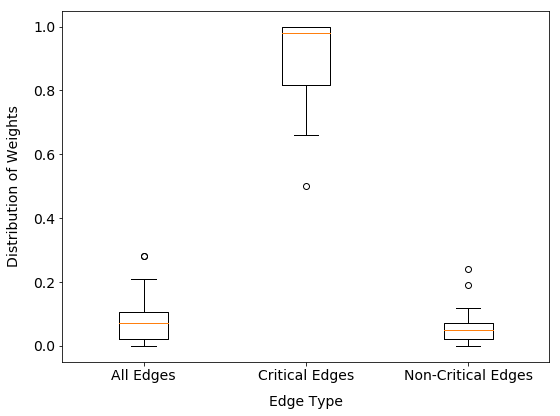
\includegraphics[width=0.48\textwidth]{figs/weight-box-avg.png}
%     \caption{Box plot showing the difference in weights between critical edges and non-critical edges.}
%     %\dcaption{All missing points distribute between $T = 0.25$ and $T = 1.0$.}
%     \label{fig:box}
% \end{figure}



\subsubsection{Revealing Critical Edges Based on Edge Weights}
\label{subsec:graphreduction}

% \begin{figure}[!ht]
%     \centering
%     \includegraphics[width=0.48\textwidth]{figs/fig:edge-thresh.pdf}
%     \caption{Effectiveness of filtering. The percentage of edges remaining after filtering drops significantly at $T = 0.10$ and remains stable below 10\%.}
%     %\dcaption{The percentage of edges remaining after filtering drops significantly at $T = 0.10$ and remains stable below 10\%.}
%     \label{fig:edge-thresh}
% \end{figure}


% \begin{figure}[!ht]
%     \centering
%     \includegraphics[width=0.48\textwidth]{figs/fig:cdf.pdf}
%     \caption{Critical edge loss from filtering. All missing points are distributed between $T = 0.25$ and $T = 1.0$.}
%     %\dcaption{All missing points distribute between $T = 0.25$ and $T = 1.0$.}
%     \label{fig:cdf}
% \end{figure}




\cref{tab:summary} shows the detailed summary of statistics of using \tool to investigate all the $18$ attack cases. 
As we can see, the number of nodes and the number of edges in the dependency graph are 412 and 19,394 on average, and can be as large as 4,252 and 151,200, while the number of critical edges are generally quite small ($<=5$), which is consistent with previous studies~\cite{mcitracking,ma2016protracer,backtracking,backtracking2}.
Thus, it is non-trivial to reveal these edges from the massive non-critical edges.

\myparatight{Edge Weight Distribution}
\cref{fig:box} shows the distribution of average weight of critical edges and non-critical edges in each case using a box plot.
We can see that the average weights of critical edges are significantly higher than that of non-critical edges. 
Note that the average weight of all edges are close to the average weight of non-critical edges because most of the edges are non-critical. 

\myparatight{Filtering Non-Critical Edges}
% The important goal of \sys is to filter out as many irrelevant edges as possible while preserving critical edges in the dependency graph.
\tool hides non-critical edges whose weights are below a threshold.
To provide a guidance on choosing this threshold, we test the filtering performance on all attack cases
%attacks studied 
in \cref{subsec:cases}
by selecting a range of values from 0.05 to 0.95 with a pace of 0.05 as 
%the 
thresholds. 
% The edges whose weights are below this number are hidden.
\cref{fig:edge-thresh} shows the average percentage of remaining edges after edge filtering. We observe that when the threshold reaches 0.10, the average percentage of remaining edges is 9.8\%, and further increasing the threshold from 0.10 to 0.90 only results in a slightly increased amount of pruned edges (2.2\%). Such results indicate that most of the edges having reputation scores below 0.10 or above 0.90. 

While a higher threshold can hide more irrelevant edges, it may cause the loss of critical edges as well.
Thus, we define the \emph{missing point} as the greatest threshold that preserves all the critical edges for a dependency graph, 
and measure the missing points for all attack cases, as shown in \cref{fig:cdf}.
We observe that:
(1) all missing points are greater than 0.25,
and (2) about 80\% of the missing points are greater than 0.90.

Combining the results in \cref{fig:edge-thresh} and \cref{fig:cdf},
we can conclude that \emph{the weight scores of almost all the critical edges are above 0.90, while the weight scores of most of the non-critical edges are below 0.10}.
Such results clearly demonstrate the effectiveness of \tool in leveraging the discriminative weights (\cref{subsec:weight-computation}) to reveal critical edges from non-critical edges.
Furthermore, based on \cref{fig:cdf}, we can suggest an optimal range of the threshold: $\lbrack 0.1,0.25 \rbrack$.
  


\eat{
% (1) Two cases (\emph{command-injection-c2}, \emph{data-leakage}) have extremely high missing points ($T_w > 200$);
% (2) 5 out of 21 cases lost critical edges at $T_w = 2$. However, in these 5 cases, 2 of them(\emph{Shell-wget},\emph{penetration-c1}) already have less than 10 non-critical edges at missing point and 3 of them also have significant reduction in edge numbers(\cref{tab:filter}).
% (3) A plateau exists before $T_w = 2$ at a rate of 24\%. This indicate most of the cases have a missing point greater than $T_w = 2$, which proves the efficacy of our weights to differ critical edges from non-critical edges.
}

\eat{
\begin{table}[]\
\centering
    	\caption{Graph reduction results for PHASEs I and II}
    	\label{tab:Reduction}
    	\resizebox{0.48\textwidth}{!}{%
            \begin{tabular}{|l|r|r|r|r|}
            \hline
            \thead{Attacks}                & \thead{PH.I V} & \thead{PH.I E} & \thead{PH.II V} & \thead{PH.II E} \\ \hline
            3File      & 225                  & 25211             & 225            & 596         \\ \hline
            2File             & 221                  & 21100             & 221            & 537         \\ \hline
            curl                  & 212                  & 15142             & 212            & 460         \\ \hline
            shell\_script           & 229                  & 21124             & 229            & 637         \\ \hline
            python\_wget          & 162                  & 10597             & 162            & 283         \\ \hline
            scp                   & 60                   & 7912              & 60             & 78          \\ \hline
            shell\_wget           & 115                  & 4998              & 115            & 158         \\ \hline
            wget                  & 217                  & 19078             & 217            & 500         \\ \hline
            command-injection-c1      & 51                   & 65                & 51             & 51          \\ \hline
            command-injection-c2      & 1438                 & 9713              & 1438           & 2738        \\ \hline
            data-leakage       & 4252                 & 151200            & 4252           & 4261        \\ \hline
            password-crack-c1 & 35                   & 731               & 35             & 36          \\ \hline
            password-crack-c2 & 61                   & 2477              & 61             & 73          \\ \hline
            password-crack-c3 & 25                   & 58426             & 25             & 36          \\ \hline
            penetration-c1 & 60                   & 314               & 60             & 63          \\ \hline
            penetration-c2 & 30                   & 139               & 30             & 68          \\ \hline
            vpnfilter-c1      & 14                   & 274               & 14             & 14          \\ \hline
            vpnfilter-c2      & 16                   & 598               & 16             & 18          \\ \hline
            avg & 412.39 & 19394.39 & 412.39 & 589.28 \\ \hline
            \end{tabular}
        }
    % \dcaption{ .}
\end{table}

Thus, we evaluate the attack sequence reconstruction via two aspects:
(1) graph reduction and (2) revealing critical edge.

\myparatight{Graph Reduction}
\cref{tab:Reduction} shows the reduction in terms of the number of nodes (Columns ``PH.I V'' and ``PH.II V'') and in the number of edges  (Columns ``PH.I E'' and ``PH.II E'') after causality analysis in Phase I (\cref{subsec:graph-generation}) and edge merge in Phase II (\cref{subsec:graph-preprocessing}).
As we can see, the reduction is significant: the biggest graph generated by \tool only contains 4252 nodes and 4261 edges (``data-leakage'' in \cref{tab:Reduction}) considering the 24-hour log contains about \emph{2 billion} events.

\myparatight{Revealing Critical Edge}
}


